% =====================================================================
%  Group-Fair Stochastic Gradient Descent via Masked Optimal Transport
%  ICASSP submission -- 4 pages + 1 page references
%
%  Compile:  pdflatex main ; pdflatex main
%  Replace the local stand-in spconf.sty with the official ICASSP one
%  before submitting. Nothing in this file needs to change.
%
%  Markers you should sweep before submission:
%     %%FILLIN   -- a number or description only you can supply
%     %%CHECK    -- a claim worth re-reading against the code
% =====================================================================
\documentclass{article}
\usepackage{spconf,amsmath,amssymb,amsthm,graphicx,booktabs,multirow}
\usepackage{algorithm}
\usepackage{algpseudocode}
\usepackage[usenames,dvipsnames]{xcolor}
\usepackage{url}
\usepackage{tikz}
\usetikzlibrary{positioning,arrows.meta,fit,backgrounds}

% ---------------------------------------------------------------- macros
\newtheorem{theorem}{Theorem}
\newtheorem{lemma}[theorem]{Lemma}
\newtheorem{proposition}[theorem]{Proposition}
\newtheorem{corollary}[theorem]{Corollary}
\theoremstyle{definition}
\newtheorem{assumption}[theorem]{Assumption}
\newtheorem{remark}[theorem]{Remark}

\newcommand{\R}{\mathbb{R}}
\newcommand{\E}{\mathbb{E}}
\newcommand{\PP}{\mathbb{P}}
\newcommand{\Nn}[1]{[#1]}
\newcommand{\simplex}[1]{\Delta^{#1-1}}
\newcommand{\CVaR}{\mathrm{CVaR}}
\newcommand{\KL}{\mathrm{KL}}
\newcommand{\Proj}{\Pi_{\mathcal{C}}}
\newcommand{\avot}{\textsf{GAVOT}}
\newcommand{\avotcvar}{\textsf{GAVOT+CVaR}}
\DeclareMathOperator*{\argmin}{arg\,min}
\DeclareMathOperator*{\argmax}{arg\,max}

\newcommand{\best}[1]{\textbf{#1}}

% ---------------------------------------------------------------- title
\title{Group-Fair Stochastic Gradient Descent \\ via Masked Optimal Transport}

\name{Herlock (SeyedAbolfazl) Rahimi \qquad Dionysis Kalogerias%
\thanks{This work is supported by NSF under Grant 2242215.}}
\address{Department of Electrical and Computer Engineering, Yale University, New Haven, CT, USA\\
\texttt{\{herlock.rahimi, dionysis.kalogerias\}@yale.edu}}

\begin{document}
\ninept
\maketitle

\begin{abstract}
Minibatch SGD is group-blind. Which groups appear in a batch is decided by how
often they occur in the data, not by how much they are meant to count in the
objective, and when the two disagree the iterates converge to a
prevalence-weighted surrogate rather than to the target risk. The gap is a bias,
so no amount of training removes it. A minibatch is a partial-participation
event over groups, which makes group-fair training an instance of federated
aggregation under availability skew, and we carry the masked optimal transport
construction of \textsf{FedAVOT} across. Aligning the
batch-composition distribution $q$ with the target importance distribution $p$
produces per-batch group weights whose induced stochastic subgradient is exactly
unbiased for the target risk, giving the standard $O(1/\sqrt{T})$ rate in the
nonsmooth convex regime with a constant that does not depend on how many groups
a batch happens to cover. Exact alignment is feasible precisely under a Hall-type condition, which reduces
to the per-group requirement that importance not exceed observation rate; past
it Sinkhorn returns an information projection and a residual we compute in
closed form rather than bound. That closed form turns the excess risk into two
terms, an alignment gain fixed by the instance and an optimization residual paid
by the estimator, and a severity sweep over eleven availability skews on Adult
and IMDb-Wiki shows the two crossing: transport wins while the gain exceeds the
residual and loses past it, at a threshold the decomposition locates in advance.
The residual is a stepsize artifact, not a property of the method, and a
decaying schedule removes it on every instance where it had reversed the sign.
A mean--CVaR layer composed on top reaches the worst group at rate
$O(\kappa(\alpha,\gamma)/\sqrt{T})$.
\end{abstract}

\begin{keywords}
Group fairness, optimal transport, stochastic gradient descent,
distribution shift, conditional value at risk.
\end{keywords}

% =====================================================================
\section{Introduction}
% =====================================================================

A classifier is rarely asked to minimize one risk. It is asked to minimize one
while behaving acceptably on subpopulations the training distribution
under-represents: a diagnostic model across patient groups, a recognition system
across demographic strata \cite{buolamwini2018gender,hashimoto2018repeated,%
sagawa2020dro}. The standard response is to change the objective, replacing the
empirical risk by $F_p(\theta)=\sum_i p_i f_i(\theta)$ with $p$ the weighting
one actually wants, uniform, inverse to prevalence, or externally dictated
\cite{mohri2019agnostic,li2020fair}.

This paper is about a gap between writing that objective down and optimizing it.
Minibatch SGD does not see $p$: it sees a batch, whose group composition is
governed by prevalence and by the sampler, so averaging the per-example
gradients descends a different function. The estimator is not merely noisy, it
is biased, by a fixed vector that survives $T\to\infty$ and any stepsize
schedule. Rebalancing the sampler is the usual and only partial fix: a group
whose prevalence is below the resolution of the batch size cannot be sampled
into every batch however the sampler is tilted, and upscaling the few examples
that do appear reintroduces an amplitude distortion that destabilizes the
iterates \cite{rahimi2025fedavot}.

\noindent\textbf{Groups as clients.}
The same mismatch is the central object of a different literature. In federated
learning the \emph{availability distribution} $q$ over which clients participate
in a round rarely matches the \emph{importance distribution} $p$ that defines
the objective, and \textsf{FedAvg} consequently optimizes a surrogate whose
weights are induced by the availability process rather than chosen
\cite{rahimi2025agnostic,wang2020objective,cho2022biased}. \textsf{FedAVOT}
\cite{rahimi2025fedavot} removes that mismatch by posing aggregation as a masked
optimal transport (MOT) problem: find a coupling whose column marginal is the
availability law and whose row marginal is the target $p$, supported only on
client-round pairs that actually occurred. The observation driving this paper is that a minibatch is a participation
event: the groups represented in $B^t$ are the active set $S^t$, its law is $q$,
and the weighting one wants is $p$. Group-fair SGD is federated aggregation with
the federation collapsed onto one machine. We call the method \avot{} and keep
the \textsf{FedAVOT} label in figures, the aggregation rule being unchanged.

\noindent\textbf{Contributions.}
\begin{enumerate}\itemsep0pt\parskip0pt\topsep2pt
\item \emph{The reduction} (Sec.~\ref{sec:setup}). Group-blind minibatch SGD reduces, under
uniform-within-batch averaging, to agnostic \textsf{FedAvg} with one local step, so the surrogate identity of
\cite{rahimi2025agnostic} names the function SGD actually minimizes, and
transport weights make the batch subgradient exactly unbiased for $\nabla F_p$
(Lemma~\ref{lem:unbiased}).
\item \emph{A coverage law and a severity measure} (Cor.~\ref{cor:batchsize}).
Feasibility is Hall-type and reduces on singletons to $p_i\le r_i$, importance
below observation rate, so the \emph{infeasible mass}
$\nu\triangleq\sum_{i:p_i>r_i}p_i$ is the natural severity axis, computable
before training.
\item \emph{A two-term decomposition that locates the crossover}
(Thm.~\ref{thm:infeasible}, Sec.~\ref{sec:exp}). Past the Hall condition the
excess splits into an \emph{alignment gain} $\Delta_{\mathrm{floor}}$, the
distance between the two optima each rule actually converges to, and an
optimization residual. The gain is exact and instance-fixed; the residual is
paid by the estimator. We sweep eleven skews and watch the two cross.
\item \emph{Risk-averse layer} (Sec.~\ref{sec:cvar}). Mean--CVaR over groups
composes with the transport weights without disturbing unbiasedness, at rate
$O(\kappa(\alpha,\gamma)/\sqrt{T})$,
$\kappa(\alpha,\gamma)=\gamma+(1-\gamma)/\alpha$.
\end{enumerate}

\noindent\textbf{Related work.}
Reduction methods for group fairness return randomized mixtures or carry an
approximation constant tied to a fixed class
\cite{agarwal2018reductions,cotter2019twoplayer,chamon2020pacc}.
Distributionally robust and worst-group objectives
\cite{sagawa2020dro,hashimoto2018repeated,levy2020large} change the functional
rather than the sampler and are complementary: our CVaR layer is one such
functional, obtained on top of transport rather than instead of it. Importance
sampling for SGD \cite{rizk2021importance,katharopoulos2018not} corrects
variance, not the identity of the minimized objective.

% =====================================================================
\section{Group-Blind SGD and its Surrogate}
\label{sec:setup}
% =====================================================================

\noindent\textbf{Setup.}
Let $\mathcal{X}\subseteq\R^d$ be a feature space, $\mathcal{Y}$ a label space,
and let the population be partitioned into $N$ groups indexed by $i\in\Nn{N}$
with prevalences $\pi\in\simplex{N}$, $\pi_i=\PP[\text{group }i]$. Group $i$
carries a distribution $\mathcal{D}_i$ on $\mathcal{X}\times\mathcal{Y}$ and a
risk
\[
f_i(\theta)\;\triangleq\;\E_{(X,Y)\sim\mathcal{D}_i}\big[\ell(m(X;\theta),Y)\big],
\qquad \theta\in\mathcal{C}\subseteq\R^{d'},
\]
with $\mathcal{C}$ convex and compact. Fix a target importance distribution
$p\in\simplex{N}$ and write
\begin{equation}
F_p(\theta)\;\triangleq\;\sum_{i=1}^{N}p_i f_i(\theta),
\qquad
\theta^\star\in\argmin_{\theta\in\mathcal{C}}F_p(\theta).
\label{eq:target}
\end{equation}
Uniform $p$ is the category-uniform objective, $p_i\propto 1/\pi_i$ the
inverse-prevalence one, and $p$ may equally be imposed externally. Throughout,
$\ell$ is convex in its first argument, bounded by $M$, with stochastic
subgradients bounded in second moment by $G^2$ on $\mathcal{C}$, and
$D\triangleq\mathrm{diam}(\mathcal{C})$.

\noindent\textbf{What a batch is.}
At step $t$ the sampler draws a batch $B^t$; write
$A^t\triangleq\{i: B^t\ \text{contains an example from group }i\}$, let
$\{A_j\}_{j\in\Nn{M}}$ enumerate the support of $A^t$ and
$q_j\triangleq\PP[A^t=A_j]$. The group-blind update assigns group $i\in A^t$ the
weight $\widehat{\pi}^t_i$, its share of the batch. The following is
\cite[Eq.~2]{rahimi2025fedavot} read at one local step, and it names the
function SGD is in fact minimizing.

\begin{proposition}[Surrogate objective]
\label{prop:surrogate}
Group-blind minibatch SGD is a stochastic subgradient method on $F_{\tilde p}$,
$\tilde p_i=\sum_{A\ni i}q(A)\E[\widehat{\pi}^t_i\mid A^t=A]$ (a probability
vector), which is $\pi$
for i.i.d.\ sampling and $\sum_{A\ni i}q(A)/|A|$ for uniform-within-batch
averaging. Consequently, for every $\theta$,
\begin{equation}
\big|F_p(\theta)-F_{\tilde p}(\theta)\big|\;\le\;M\|p-\tilde p\|_1 ,
\label{eq:surrogate-gap}
\end{equation}
and the excess risk of any method that minimizes $F_{\tilde p}$ exactly is at
least $F_p(\theta^\star_{\tilde p})-F_p(\theta^\star)$, which is bounded above
by $2M\|p-\tilde p\|_1$ and does not vanish with $T$.
\end{proposition}

The content of Proposition~\ref{prop:surrogate} is that the choice of $p$ in
\eqref{eq:target} is decorative unless the aggregation step is changed, and that
tilting the sampler so that $\tilde p=p$ is available only when $p$ is
reachable, which is the question the next section answers.

% =====================================================================
\section{Alignment by Masked Optimal Transport}
\label{sec:gavot}
% =====================================================================

\noindent\textbf{The coupling.}
Let $Y[i,j]$ be the weight assigned to group $i$ when the batch composition is
$A_j$, and let $T[i,j]\triangleq q_j Y[i,j]$ be the joint mass. Requiring that
the weights be a probability vector on each realized composition, and that they
reproduce $p$ in expectation, is
\begin{equation}
T\mathbf{1}_M=p,\qquad \mathbf{1}_N^\top T=q,\qquad T\ge 0,
\qquad \mathrm{supp}(T)\subseteq E,
\label{eq:mot}
\end{equation}
with mask $E=\{(i,j): i\in A_j\}$ encoding that a group absent from the batch
cannot be weighted. This is a feasibility problem, not a cost minimization:
any coupling respecting \eqref{eq:mot} serves. Fig.~\ref{fig:mask} is the
picture.

\begin{figure}[t]
\centering
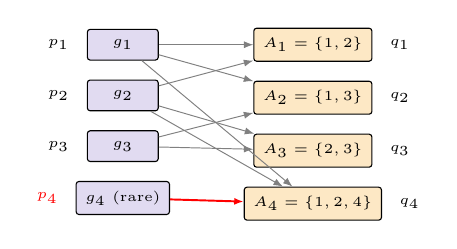
\begin{tikzpicture}[
   node distance=2.4mm,
   grp/.style={draw,rounded corners=1pt,minimum width=9mm,minimum height=3.9mm,font=\tiny,fill=Periwinkle!20},
   atm/.style={draw,rounded corners=1pt,minimum width=13mm,minimum height=3.9mm,font=\tiny,fill=YellowOrange!20},
   e/.style={-{Latex[length=1.2mm]},gray,line width=.35pt},
   lbl/.style={font=\tiny\itshape}
]
\node[grp] (g1) {$g_1$};
\node[grp,below=of g1] (g2) {$g_2$};
\node[grp,below=of g2] (g3) {$g_3$};
\node[grp,below=of g3] (g4) {$g_4$ \tiny(rare)};

\node[atm,right=12mm of g1] (a1) {$A_1=\{1,2\}$};
\node[atm,below=of a1] (a2) {$A_2=\{1,3\}$};
\node[atm,below=of a2] (a3) {$A_3=\{2,3\}$};
\node[atm,below=of a3] (a4) {$A_4=\{1,2,4\}$};

\draw[e] (g1)--(a1); \draw[e] (g2)--(a1);
\draw[e] (g1)--(a2); \draw[e] (g3)--(a2);
\draw[e] (g2)--(a3); \draw[e] (g3)--(a3);
\draw[e] (g1)--(a4); \draw[e] (g2)--(a4); \draw[e,Red,line width=.7pt] (g4)--(a4);

\node[lbl,left=1mm of g1] {$p_1$};
\node[lbl,left=1mm of g2] {$p_2$};
\node[lbl,left=1mm of g3] {$p_3$};
\node[lbl,left=1mm of g4,Red] {$p_4$};
\node[lbl,right=1mm of a1] {$q_1$};
\node[lbl,right=1mm of a2] {$q_2$};
\node[lbl,right=1mm of a3] {$q_3$};
\node[lbl,right=1mm of a4] {$q_4$};
\end{tikzpicture}
\caption{The mask $E$. Batch compositions carry the mass $q$ they occur with;
groups must receive the mass $p$ the objective assigns them. Group $4$ is
reachable only through $A_4$, so exact alignment requires $p_4\le q_4$: the
Hall condition of Thm.~\ref{thm:feas} read on the singleton $I=\{4\}$. Shrinking
the batch deletes $A_4$ from the support and makes $p_4$ unreachable.}
\label{fig:mask}
\end{figure}

\begin{theorem}[Feasibility, {\cite[Thm.~1]{rahimi2025fedavot}}]
\label{thm:feas}
For $I\subseteq\Nn{N}$ let $\mathcal{N}(I)=\{j:\exists\,i\in I,\ (i,j)\in E\}$
and $\mathcal{S}(I)=\{j: A_j\subseteq I\}$. Problem \eqref{eq:mot} is feasible
if and only if
$\sum_{j\in\mathcal{S}(I)}q_j\le\sum_{i\in I}p_i\le\sum_{j\in\mathcal{N}(I)}q_j$
for every $I\subseteq\Nn{N}$.
\end{theorem}

On singletons it becomes a statement one can act on before training starts.

\begin{corollary}[Coverage law and severity]
\label{cor:batchsize}
Feasibility of \eqref{eq:mot} requires $\PP[A^t=\{i\}]\le p_i\le r_i$ for every
$i$, where $r_i\triangleq\PP[i\in A^t]$ is the observation rate of group $i$.
Writing
\begin{equation}
\nu\;\triangleq\!\!\sum_{i\,:\,p_i>r_i}\!\! p_i
\label{eq:batchlaw}
\end{equation}
for the \emph{infeasible mass}, $\nu=0$ iff the upper coverage constraints hold.
Under i.i.d.\ sampling of $b$ examples with prevalences $\pi$ this reads
$b\ge\log(1-p_i)/\log(1-\pi_i)$; under $K$-of-$N$ uniform group sampling it
reads $p_i\le K/N$.
\end{corollary}

\noindent\textbf{Severity.}
The infeasible mass $\nu$ of \eqref{eq:batchlaw} is the axis we sweep. At
$\nu=0$ every group is observed at least as often as its importance and exact
alignment is available; as $\nu$ grows, more of $p$ sits outside the reachable
polytope. Reporting a \emph{feasible} and an \emph{infeasible} regime is
therefore reporting two points on a continuum, and Sec.~\ref{sec:exp} sweeps it
instead.

\noindent\textbf{Computing the plan.}
Given feasibility, $T$ is obtained by iterative proportional fitting (Sinkhorn
scaling) on the masked support \cite{sinkhorn1967,cuturi2013,peyre2019}. It is
computed once, offline, at $O(|E|)$ per sweep with $|E|\le NM$ and $M$ the
number of realized compositions rather than $2^N$; the loop adds one lookup and
one multiply per group per step. Since $\mathbf{1}_N^\top T=q$ and
$Y=T\mathrm{diag}(q)^{-1}$, every column $Y[\cdot,j]$ is a probability vector on
$A_j$, the property each bound below uses.

\begin{algorithm}[t]
\caption{\avot{}: group-fair SGD by masked transport}
\label{alg:gavot}
\begin{algorithmic}[1]
\Require target $p$, composition law $(q,\{A_j\},E)$, step $\eta$, horizon $T$,
 CVaR parameters $(\alpha,\gamma)$ with $\gamma=1$ for the risk-neutral method
\State $(T,Y)\leftarrow$ Sinkhorn scaling for $(p,q,E)$ \Comment{offline, once}
\State $\theta^0\in\mathcal{C}$, $\ t^0\in\R$
\For{$t=1,\dots,T$}
  \State draw batch $B^t$; set $A^t$, let $j(t)$ be s.t.\ $A_{j(t)}=A^t$
  \State $g^t_i \leftarrow$ stochastic subgradient of $f_i$ from $B^t\cap$ group $i$
  \State $w^t_i \leftarrow Y[i,j(t)]\big(\gamma+\tfrac{1-\gamma}{\alpha}\mathbf{1}\{\hat f^t_i>t^{t-1}\}\big)$
  \State $\theta^{t}\leftarrow\Proj\big(\theta^{t-1}-\eta\sum_{i\in A^t}w^t_i\,g^t_i\big)$
  \State $t^{t}\leftarrow t^{t-1}-\eta(1-\gamma)\big(1-\tfrac{1}{\alpha}\sum_{i\in A^t}Y[i,j(t)]\mathbf{1}\{\hat f^t_i>t^{t-1}\}\big)$
\EndFor
\Ensure $\bar\theta_T=\frac{1}{T}\sum_{t=1}^{T}\theta^t$
\end{algorithmic}
\end{algorithm}

\noindent\textbf{Why it works.}
Everything rests on one identity, \cite[Lem.~1]{rahimi2025fedavot} moved from
model averaging to gradient averaging. Transport removes bias; it is not a
variance reduction device.

\begin{lemma}[Unbiasedness]
\label{lem:unbiased}
Let $T$ satisfy \eqref{eq:mot} and $\hat g(\theta)=\sum_{i\in A^t}Y[i,j(t)]g_i(\theta)$.
Then $\E[\hat g(\theta)\mid\theta]\in\partial F_p(\theta)$ for every
$\theta\in\mathcal{C}$.
\end{lemma}
\begin{proof}
Taking expectation over $A^t\sim q$ and then over the minibatch noise,
$\E[\hat g]=\sum_{A}q(A)\sum_i Y[i,j(A)]\mathbf{1}\{i\in A\}\,\nabla f_i(\theta)
=\sum_i\big(\sum_j T[i,j]\big)\nabla f_i(\theta)=\sum_i p_i\nabla f_i(\theta)$,
the row-marginal constraint being used in the last step.
\end{proof}

\begin{lemma}[Second moment, free of coverage]
\label{lem:variance}
$\E\|\hat g(\theta)\|^2\le G^2$ for every $\theta\in\mathcal{C}$, with no
dependence on $|A^t|$ or on $N$.
\end{lemma}
\begin{proof}
$Y[\cdot,j]$ is a probability vector on $A_j$, so
$\|\sum_i Y[i,j]g_i\|^2\le\sum_i Y[i,j]\|g_i\|^2$ by convexity; take
expectations and use the row-marginal identity of Lemma~\ref{lem:unbiased}.
\end{proof}

\begin{theorem}[Rate]
\label{thm:rate}
Let $f_i$ be convex, $\mathcal{C}$ convex compact, and let \eqref{eq:mot} be
feasible. Algorithm~\ref{alg:gavot} with $\gamma=1$ and
$\eta=D/(G\sqrt{T})$ satisfies
\begin{equation}
\E\big[F_p(\bar\theta_T)\big]-F_p(\theta^\star)\;\le\;\frac{DG}{\sqrt{T}} .
\end{equation}
The constant is independent of how many groups appear in a batch: a composition
covering two groups yields the same bound as one covering all $N$, though with
larger realized variance.
\end{theorem}
\begin{proof}
By Lemmas~\ref{lem:unbiased} and~\ref{lem:variance} the iteration is projected
stochastic subgradient descent on the convex $F_p$ with an unbiased oracle of
second moment at most $G^2$ \cite{nemirovski2009}; no step refers to $|A^t|$.
\end{proof}

\noindent\textbf{Outside the feasible region.}
When the Hall condition fails, \eqref{eq:mot} has no solution and Sinkhorn does
not diverge: its iterates accumulate at the coupling whose reachable row
marginal $\hat p$ is the KL-closest to $p$ over the polytope
$\{T\ge 0:\ \mathbf{1}^\top T=q,\ \mathrm{supp}(T)\subseteq E\}$
\cite{csiszar1975,gietl2013ipfp,peyre2019}. The column marginal is met exactly, so
Lemmas~\ref{lem:unbiased} and~\ref{lem:variance} hold with $p$ replaced by
$\hat p$, and the loss is a bias of exactly the shape of
Proposition~\ref{prop:surrogate}.

\begin{theorem}[Infeasible regime]
\label{thm:infeasible}
Let $\hat p$ be the row marginal of the Sinkhorn limit and write
$\Phi(w)\triangleq F_p\big(\argmin_\theta F_w(\theta)\big)$ for the $p$-risk of
the minimizer of the $w$-weighted risk. Then
\begin{equation}
\E\big[F_p(\bar\theta_T)\big]-F_p(\theta^\star)
\;=\;\underbrace{\Phi(\hat p)-\Phi(p)}_{\text{alignment floor}}
\;+\;\underbrace{\varepsilon_T(\hat p)}_{\text{optimization residual}} ,
\label{eq:infeasible}
\end{equation}
and group-blind averaging obeys \eqref{eq:infeasible} with $\tilde p$ for
$\hat p$. Writing $\Delta_{\mathrm{floor}}\triangleq\Phi(\tilde p)-\Phi(\hat p)$
for the alignment gain, transport improves on group-blind averaging exactly
when $\Delta_{\mathrm{floor}}>\varepsilon_T(\hat p)-\varepsilon_T(\tilde p)$.
The floors are bounded by $\Phi(w)-\Phi(p)\le 2M\|p-w\|_1$.
\end{theorem}
\begin{proof}
The floor term is $F_p$ evaluated at the two limits and is exact by definition.
Theorem~\ref{thm:rate} applied to $F_{\hat p}$ bounds its suboptimality by
$DG/\sqrt{T}$; $\varepsilon_T$ also carries the $p$-versus-$\hat p$ mismatch
along the trajectory, vanishing as $\bar\theta_T\to\theta^\dagger$.
The $\ell_1$ bound follows from $0\le f_i\le M$ as in
Proposition~\ref{prop:surrogate}.
\end{proof}

Both terms of \eqref{eq:infeasible} are available before training: $\hat p$ and
$\tilde p$ from $(p,q,E)$, and on instances with a closed-form frontier
$\Phi$ exactly. The $\ell_1$ bound is the weaker object and we report both,
because it turns out to be too loose to discriminate.

% =====================================================================
\section{A Risk-Averse Layer over Groups}
\label{sec:cvar}
% =====================================================================

Exact alignment delivers the $p$-weighted risk, an average, which can hide a
group. Where the requirement is on the worst group instead, we compose a
mean--CVaR functional over groups on top of the transport weights
\cite{rahimi2025agnostic,rockafellar2000cvar}:
\begin{equation}
F_p^{\alpha,\gamma}(\theta)\;\triangleq\;\gamma F_p(\theta)+(1-\gamma)\,
\CVaR^p_\alpha\big(f(\theta)\big),\quad \alpha,\gamma\in(0,1],
\label{eq:meancvar}
\end{equation}
where $\CVaR^p_\alpha$ is the conditional value at risk of the group-loss vector
under $p$. The Rockafellar--Uryasev representation turns \eqref{eq:meancvar}
into a joint minimization over $(\theta,t)$,
\begin{equation}
\Phi(\theta,t)=\gamma\sum_i p_i f_i(\theta)+(1-\gamma)\Big(t+\tfrac{1}{\alpha}
\sum_i p_i\big[f_i(\theta)-t\big]_+\Big),
\label{eq:ru}
\end{equation}
jointly convex, with subgradients in both arguments again $p$-weighted sums of
per-group quantities, so Lemma~\ref{lem:unbiased} applies unchanged. This is why
the layers compose rather than interfere: transport fixes \emph{which}
distribution the expectation is under, CVaR changes \emph{what} is averaged.
Lines 6 and 8 of Algorithm~\ref{alg:gavot} implement \eqref{eq:ru}.

\begin{theorem}[Rate under mean--CVaR]
\label{thm:cvar}
Under the hypotheses of Theorem~\ref{thm:rate}, Algorithm~\ref{alg:gavot} with
$\eta=\Theta(1/\sqrt{T})$ satisfies
$\E[F_p^{\alpha,\gamma}(\bar\theta_T)]-\min F_p^{\alpha,\gamma}
=O\!\big(\kappa(\alpha,\gamma)/\sqrt{T}\big)$ with
$\kappa(\alpha,\gamma)=\gamma+(1-\gamma)/\alpha$. In the infeasible regime the
bound of Theorem~\ref{thm:infeasible} acquires the same factor on its
statistical term, the bias term being unchanged.
\end{theorem}

Both $\gamma=1$ and $\alpha=1$ recover Theorem~\ref{thm:rate} exactly, so the
grid contains the risk-neutral method along two edges, visible as the constant
row and column of every heatmap below. Sending $\alpha\downarrow 0$ drives
\eqref{eq:meancvar} to the worst group at the cost
$\kappa(\alpha,\gamma)\to\infty$: the parameter prices robustness in the
convergence constant, not in the limit.

\begin{remark}[Relation to constrained learning]
\label{rem:penalty}
$\max_i f_i$ is the exact-penalty limit of $\min f_0$ s.t.\ $f_i\le c_i$, a
fixed price on the largest violation matching penalized and constrained values
once it exceeds the least $\ell_1$ norm on the dual-optimal set
\cite{rahimi2026exactpenalty}. The $\alpha\downarrow 0$ edge of
\eqref{eq:meancvar} is thus the scalarization a constrained specification
selects, with $\kappa$ its price in the rate.
\end{remark}

% =====================================================================
\section{Experiments}
\label{sec:exp}

\noindent\textbf{Instances.}
\emph{Adult} income classification \cite{uci_adult} (logistic regression,
$\eta{=}0.1$) with a uniform importance target over the five race groups, $100$
race-homogeneous groups of $30$ samples split $85/10/3/1/1$ by prevalence, and
\emph{IMDb-Wiki} age regression \cite{rothe2018imdbwiki} (linear regression on
ResNet embeddings, $\eta{=}10^{-2}$) over $100$ identities with a cubically
skewed importance target. Both use $K=3$ observed groups per step,
$H{=}5$ local steps per observed group before the weighted average, $4000$
steps, $5$ seeds, tail-500 statistics. Availability rates $r$ are swept through
a family indexed by $\beta$, from prevalence-proportional to importance-aligned
on Adult and through increasing skew on IMDb-Wiki, giving eleven instances whose
infeasible mass $\nu$ of \eqref{eq:batchlaw} ranges from $0$ to $88\%$. On both
the perturbation frontier is closed-form, so the floors $\Phi(p),\Phi(\hat p),
\Phi(\tilde p)$ of Theorem~\ref{thm:infeasible} are exact rather than estimated.
Besides group-blind averaging we include the fixed multiplier $m/K$, the
rescaling that assumes a uniform observation rate.

% ----------------------------------------------------------- Table 1
\begin{table}[t]
\centering
\caption{Headline cells, tail-500 over $5$ seeds, decaying stepsize. \emph{full}
sees every group every step. The fixed multiplier $m/K$ diverges whenever
observation rates are non-uniform.}
\label{tab:overall}
\setlength{\tabcolsep}{2.4pt}
\begin{tabular}{lcccc}
\toprule
Instance & \avot{} & unif.\ avg & $m/K$ & full \\
\midrule
Adult, prevalence ($\nu{=}.60$) & $\best{0.2269}$ & $0.2479$ & $0.670$ & $0.2073$ \\
Adult, aligned ($\nu{=}0$)      & $0.2075$ & $0.2077$ & div. & $0.2073$ \\
IMDb, skewed ($\nu{=}.31$)      & $\best{86.06}$ & $91.63$ & $8504$ & $82.95$ \\
IMDb, aligned ($\nu{=}0$)       & $\best{84.28}$ & $86.37$ & div. & $82.95$ \\
\bottomrule
\end{tabular}
\end{table}

% ----------------------------------------------------------- Fig 2
\begin{figure}[t]
\centering
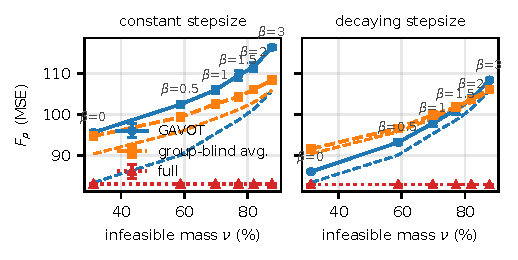
\includegraphics[width=0.92\columnwidth]{figs/severity_imdb.pdf}
\caption{IMDb-Wiki severity sweep. Solid, measured tail-500 ($\pm1$ std);
dashed, the exact floor $\Phi(\cdot)$ each rule converges to. Left, constant
stepsize: the optimization residual swamps the alignment gain and transport
loses everywhere, even where the floors are seven units apart. Right, decaying
stepsize: the residual collapses and the measured curves track their floors, so
transport wins until the floors close at high $\nu$. The sign is set by which of
the two terms of \eqref{eq:infeasible} dominates, not by the regime label.}
\label{fig:severity}
\end{figure}

\noindent\textbf{E1: the headline cells.}
Table~\ref{tab:overall} reports the four instances a practitioner would
recognize. Transport wins on three: Adult under prevalence-proportional
availability, $0.2269$ against $0.2479$ ($t{=}45$), and both IMDb cells,
$86.06$ against $91.63$ ($t{=}21$) and $84.28$ against $86.37$ ($t{=}13$). On
Adult with importance-aligned availability the two coincide at the oracle
value, which is what Proposition~\ref{prop:surrogate} predicts when
$\tilde p=p$: there is nothing to correct and transport does not manufacture a
difference. The fixed multiplier diverges on both aligned instances and is far
off on the other two, so naive rescaling is no alternative to solving \eqref{eq:mot}.

% ----------------------------------------------------------- Table 2
\begin{table}[t]
\centering
\caption{IMDb-Wiki severity sweep, decaying stepsize. $\Delta_{\mathrm{floor}}$
is the alignment gain of Theorem~\ref{thm:infeasible}, \emph{gain} the measured
advantage of transport, $t$ its Welch statistic (population std). The excess
residual transport pays averages $1.9$, and the sign flips exactly where
$\Delta_{\mathrm{floor}}$ crosses it. The five Adult skews all sit above their
crossover and are omitted.}
\label{tab:severity}
\setlength{\tabcolsep}{3.0pt}
\begin{tabular}{ccccc}
\toprule
$\beta$ & $\nu$ & $\Delta_{\mathrm{floor}}$ & gain & $t$ \\
\midrule
$0$   & $.31$ & $6.99$ & $\best{+5.57}$ & $20.7$ \\
$0.5$ & $.59$ & $5.71$ & $\best{+3.46}$ & $11.3$ \\
$1.0$ & $.70$ & $3.67$ & $\best{+2.05}$ & $5.4$ \\
$1.5$ & $.77$ & $2.56$ & $+0.58$ & $1.1$ \\
$2.0$ & $.82$ & $1.62$ & $-0.03$ & $-0.1$ \\
$3.0$ & $.88$ & $0.02$ & $-2.28$ & $-7.9$ \\
\bottomrule
\end{tabular}
\end{table}

\noindent\textbf{E2: the crossover, and where the sign comes from.}
Table~\ref{tab:severity} and Fig.~\ref{fig:severity} are the paper's main
evidence. On Adult, whose five skews are omitted from the table, the measured gain tracks
$\Delta_{\mathrm{floor}}$ within $4\%$ at three of five
($.0134$ against $.0129$, $.0050$ against $.0049$, $.0002$ against $.0003$)
and exceeds it at the two most infeasible ($.0210$ against $.0110$, $.0181$
against $.0144$), group-blind averaging sitting further above its floor. On IMDb-Wiki the gain is
uniformly below the floor by an excess optimization residual that is close to
constant in $\beta$, mean $1.9$ in MSE units, and the measured sign flips
precisely where $\Delta_{\mathrm{floor}}$ crosses that value, between
$\beta{=}1.5$ ($2.56$, gain $+0.58$) and $\beta{=}2.0$ ($1.62$, gain $-0.03$).
This is Theorem~\ref{thm:infeasible} read at finite $T$: the sign of the
comparison is a quantity one computes in advance.

\noindent\textbf{E3: the $\ell_1$ bound is too loose to be the criterion.}
The distances $\|p-\hat p\|_1$ and $\|p-\tilde p\|_1$ are also computed on every
instance, and $\|p-\hat p\|_1<\|p-\tilde p\|_1$ holds in all eleven, including
the three where transport loses or ties. The $\ell_1$ form of
Theorem~\ref{thm:infeasible} therefore never predicts a loss and cannot serve as
the criterion; the exact floors can.

\noindent\textbf{E4: the residual is a stepsize artifact.}
The left panel of Fig.~\ref{fig:severity} runs the identical instances at
constant stepsize. There transport loses on all six IMDb skews, by as much as
$7.9$, even at $\nu{=}.31$ where the floors are $6.99$ apart. The transport
weights $Y[\cdot,j]$ concentrate mass on rarely observed groups, so although
Lemma~\ref{lem:variance} bounds the second moment identically for both rules,
the variance about the mean is larger, and at constant stepsize the iterates sit
on a noise floor proportional to it. Under $\eta_t=\eta/(1+t/1000)$ that floor
decays, the measured curves fall onto their dashed floors, and every sign
reversal attributable to the stepsize disappears. The residual is a property of
the schedule, not of the estimator.

\noindent\textbf{E5: risk aversion, and where it does not help.}
Sweeping $(\alpha,\gamma)$ on a $10\times10$ grid, the overall objective is
minimized on the $\gamma=1$ edge on every instance, which is
$\kappa(1,\gamma)=1$ made visible and confirms that risk aversion costs the
average. The one place the CVaR layer earns its keep is the worst race on Adult
under prevalence availability, where \avotcvar{} at $(0.2,0.7)$ reaches
$0.3624$ against $0.3679$ for \avot{} and $0.3994$ for group-blind averaging.
Per race, transport improves four of five (Black $.179$ vs $.200$, Asian-Pac
$.368$ vs $.399$, Am-Ind $.175$ vs $.189$, Other $.073$ vs $.119$) and regresses
only the majority group ($.339$ vs $.332$), which is what reweighting toward a
category-uniform target is supposed to do.

% =====================================================================
\section{Conclusion}
% =====================================================================

Group-fair training fails in a specific and fixable place: the aggregation step,
blind to the weighting the objective declares. Reading a minibatch as a
partial-participation event makes the fix the masked transport problem that
corrects availability skew in federated learning, with the same feasibility
characterization, an $O(1/\sqrt{T})$ guarantee free of batch coverage, and a
coverage law whose infeasible mass $\nu$ orders instances by severity. Past
feasibility the excess splits cleanly, into an alignment gain fixed by the
instance and an optimization residual paid by the estimator, and a sweep over
eleven skews shows the two crossing where the decomposition says they will. Transport is
worth applying while the gain exceeds the residual, both are computable before
training, and the residual is a stepsize artifact a decaying schedule removes.
The nonconvex case remains open.

% =====================================================================
\clearpage
\renewcommand{\refname}{REFERENCES}

\begin{thebibliography}{99}\setlength{\itemsep}{-1pt}\small

\bibitem{buolamwini2018gender}
J.~Buolamwini and T.~Gebru, ``Gender shades: Intersectional accuracy disparities
in commercial gender classification,'' in \emph{Proc. Conf. Fairness,
Accountability and Transparency (FAT*)}, 2018, pp. 77--91.

\bibitem{hashimoto2018repeated}
T.~Hashimoto, M.~Srivastava, H.~Namkoong, and P.~Liang, ``Fairness without
demographics in repeated loss minimization,'' in \emph{Proc. Int. Conf. Machine
Learning (ICML)}, 2018, pp. 1929--1938.

\bibitem{sagawa2020dro}
S.~Sagawa, P.~W. Koh, T.~Hashimoto, and P.~Liang, ``Distributionally robust
neural networks for group shifts,'' in \emph{Proc. Int. Conf. Learning
Representations (ICLR)}, 2020.

\bibitem{mohri2019agnostic}
M.~Mohri, G.~Sivek, and A.~T. Suresh, ``Agnostic federated learning,'' in
\emph{Proc. Int. Conf. Machine Learning (ICML)}, 2019, pp. 4615--4625.

\bibitem{li2020fair}
T.~Li, M.~Sanjabi, A.~Beirami, and V.~Smith, ``Fair resource allocation in
federated learning,'' in \emph{Proc. Int. Conf. Learning Representations
(ICLR)}, 2020.

\bibitem{rahimi2025fedavot}
H.~Rahimi and D.~Kalogerias, ``FedAVOT: Exact distribution alignment in
federated learning via masked optimal transport,'' in \emph{Proc. IEEE Int.
Conf. Acoustics, Speech and Signal Processing (ICASSP)}, 2026.

\bibitem{rahimi2025agnostic}
H.~Rahimi and D.~Kalogerias, ``Convergence of agnostic federated averaging,''
in \emph{Proc. IEEE Int. Workshop Computational Advances in Multi-Sensor
Adaptive Processing (CAMSAP)}, 2025.

\bibitem{wang2020objective}
J.~Wang, Q.~Liu, H.~Liang, G.~Joshi, and H.~V. Poor, ``Tackling the objective
inconsistency problem in heterogeneous federated optimization,'' in \emph{Adv.
Neural Inf. Process. Syst. (NeurIPS)}, vol.~33, 2020, pp. 7611--7623.

\bibitem{cho2022biased}
Y.~J. Cho, J.~Wang, and G.~Joshi, ``Towards understanding biased client
selection in federated learning,'' in \emph{Proc. Int. Conf. Artificial
Intelligence and Statistics (AISTATS)}, 2022, pp. 10351--10375.

\bibitem{mcmahan2017fedavg}
H.~B. McMahan, E.~Moore, D.~Ramage, S.~Hampson, and B.~A. y~Arcas,
``Communication-efficient learning of deep networks from decentralized data,''
in \emph{Proc. Int. Conf. Artificial Intelligence and Statistics (AISTATS)},
2017, pp. 1273--1282.

\bibitem{agarwal2018reductions}
A.~Agarwal, A.~Beygelzimer, M.~Dud\'{i}k, J.~Langford, and H.~Wallach, ``A
reductions approach to fair classification,'' in \emph{Proc. Int. Conf. Machine
Learning (ICML)}, 2018, pp. 60--69.

\bibitem{cotter2019twoplayer}
A.~Cotter, H.~Jiang, and K.~Sridharan, ``Two-player games for efficient
non-convex constrained optimization,'' in \emph{Proc. Int. Conf. Algorithmic
Learning Theory (ALT)}, 2019, pp. 300--332.

\bibitem{chamon2020pacc}
L.~F.~O. Chamon and A.~Ribeiro, ``Probably approximately correct constrained
learning,'' in \emph{Adv. Neural Inf. Process. Syst. (NeurIPS)}, vol.~33, 2020,
pp. 16722--16735.

\bibitem{chamon2023nonconvex}
L.~F.~O. Chamon, S.~Paternain, M.~Calvo-Fullana, and A.~Ribeiro, ``Constrained
learning with non-convex losses,'' \emph{IEEE Trans. Inf. Theory}, vol.~69,
no.~3, pp. 1739--1760, 2023.

\bibitem{rahimi2026exactpenalty}
H.~Rahimi, S.~Pougkakiotis, and D.~Kalogerias, ``An exact penalty method for
constrained statistical learning over universal RKHSs,'' 2026, submitted.
%%FILLIN: replace with the arXiv number once posted.

\bibitem{rizk2021importance}
M.~Rizk, S.~Vlaski, and A.~H. Sayed, ``Optimal importance sampling for
federated learning,'' in \emph{Proc. IEEE Int. Conf. Acoustics, Speech and
Signal Processing (ICASSP)}, 2021, pp. 3110--3114.

\bibitem{katharopoulos2018not}
A.~Katharopoulos and F.~Fleuret, ``Not all samples are created equal: Deep
learning with importance sampling,'' in \emph{Proc. Int. Conf. Machine
Learning (ICML)}, 2018, pp. 2525--2534.

\bibitem{sinkhorn1967}
R.~Sinkhorn, ``Diagonal equivalence to matrices with prescribed row and column
sums,'' \emph{Amer. Math. Monthly}, vol.~74, no.~4, pp. 402--405, 1967.

\bibitem{cuturi2013}
M.~Cuturi, ``Sinkhorn distances: Lightspeed computation of optimal transport,''
in \emph{Adv. Neural Inf. Process. Syst. (NeurIPS)}, vol.~26, 2013, pp.
2292--2300.

\bibitem{peyre2019}
G.~Peyr\'{e} and M.~Cuturi, \emph{Computational Optimal Transport}. Now
Publishers, 2019.

\bibitem{gietl2013ipfp}
C.~Gietl and F.~P. Reffel, ``Accumulation points of the iterative proportional
fitting procedure,'' \emph{Statistics}, vol.~47, no.~6, pp. 1321--1335, 2013.

\bibitem{csiszar1975}
I.~Csisz\'{a}r, ``$I$-divergence geometry of probability distributions and
minimization problems,'' \emph{Ann. Probab.}, vol.~3, no.~1, pp. 146--158, 1975.

\bibitem{hall1935}
P.~Hall, ``On representatives of subsets,'' \emph{J. London Math. Soc.},
vol.~10, no.~1, pp. 26--30, 1935.

\bibitem{fordfulkerson1956}
L.~R. Ford and D.~R. Fulkerson, ``Maximal flow through a network,'' \emph{Canad.
J. Math.}, vol.~8, pp. 399--404, 1956.

\bibitem{villani2009}
C.~Villani, \emph{Optimal Transport: Old and New}. Springer, 2009.

\bibitem{rockafellar2000cvar}
R.~T. Rockafellar and S.~Uryasev, ``Optimization of conditional value-at-risk,''
\emph{J. Risk}, vol.~2, no.~3, pp. 21--41, 2000.

\bibitem{curi2020adaptive}
S.~Curi, K.~Y. Levy, S.~Jegelka, and A.~Krause, ``Adaptive sampling for
stochastic risk-averse learning,'' in \emph{Adv. Neural Inf. Process. Syst.
(NeurIPS)}, vol.~33, 2020, pp. 1036--1047.

\bibitem{levy2020large}
D.~Levy, Y.~Carmon, J.~C. Duchi, and A.~Sidford, ``Large-scale methods for
distributionally robust optimization,'' in \emph{Adv. Neural Inf. Process.
Syst. (NeurIPS)}, vol.~33, 2020, pp. 8847--8860.

\bibitem{namkoong2017variance}
H.~Namkoong and J.~C. Duchi, ``Variance-based regularization with convex
objectives,'' in \emph{Adv. Neural Inf. Process. Syst. (NeurIPS)}, vol.~30,
2017, pp. 2971--2980.

\bibitem{nemirovski2009}
A.~Nemirovski, A.~Juditsky, G.~Lan, and A.~Shapiro, ``Robust stochastic
approximation approach to stochastic programming,'' \emph{SIAM J. Optim.},
vol.~19, no.~4, pp. 1574--1609, 2009.

\bibitem{li2020fedprox}
T.~Li, A.~K. Sahu, M.~Zaheer, M.~Sanjabi, A.~Talwalkar, and V.~Smith,
``Federated optimization in heterogeneous networks,'' in \emph{Proc. Machine
Learning and Systems (MLSys)}, 2020, pp. 429--450.

\bibitem{karimireddy2020scaffold}
S.~P. Karimireddy, S.~Kale, M.~Mohri, S.~J. Reddi, S.~U. Stich, and A.~T.
Suresh, ``SCAFFOLD: Stochastic controlled averaging for federated learning,''
in \emph{Proc. Int. Conf. Machine Learning (ICML)}, 2020, pp. 5132--5143.

\bibitem{uci_adult}
B.~Becker and R.~Kohavi, ``Adult,'' UCI Machine Learning Repository, 1996.

\bibitem{rothe2018imdbwiki}
R.~Rothe, R.~Timofte, and L.~Van~Gool, ``Deep expectation of real and apparent
age from a single image without facial landmarks,'' \emph{Int. J. Comput.
Vis.}, vol.~126, no.~2--4, pp. 144--157, 2018.

\bibitem{theodoropoulos2024restricted}
P.~Theodoropoulos, K.~E. Nikolakakis, and D.~Kalogerias, ``Federated learning
under restricted user availability,'' in \emph{Proc. IEEE Int. Conf. Acoustics,
Speech and Signal Processing (ICASSP)}, 2024.

\end{thebibliography}

\end{document}
